\documentclass[12pt]{report}

\usepackage{url}
\usepackage[utf8]{inputenc} % This defines the font-encoding you prefer to use
\usepackage[pdftex]{graphicx}
\usepackage[bindingoffset=1cm,centering,includeheadfoot,margin=2cm]{geometry}

\usepackage[
    citestyle=numeric-comp,
    backend=biber,
    bibencoding=inputenc
    ]{biblatex}
\addbibresource{refs.bib}

\usepackage{setspace}
\linespread{1.5}
\setcounter{tocdepth}{2}
\usepackage[colorlinks=true, pdfstartview=FitV,
linkcolor=blue, citecolor=blue, urlcolor=blue]{hyperref}
\setlength{\parindent}{0pt} % No indentation between paragraphs
\setlength{\parskip}{10pt} % Space between paragraphs

% Tables
\usepackage{ltxtable}
\usepackage{booktabs}

% Needed for code listings
\usepackage{listings}
\usepackage{color}

% Subfigure
\usepackage{subcaption}
\usepackage{floatpag} % to move floatpagenr to topright

% Fußnote
\usepackage[hang]{footmisc}
\setlength{\footnotemargin}{-0.8em}

\usepackage{csquotes}
\usepackage{afterpage} % needed for empty page after front

\usepackage[all]{nowidow} % prevents overhanging paragraphs
\usepackage{acronym} % allow acronyms

%%===================================
% Custom definitions
    
% Signal color
\definecolor{signalColor}{RGB}{164, 63, 114}
\newcommand\signal[1]{\textbf{\textcolor{signalColor}{#1}}}
    
% List with less space between items
\newenvironment{cList}{
\begin{itemize}
  \setlength{\itemsep}{0pt}
  \setlength{\parskip}{0pt}
  \setlength{\parsep}{0pt}
}{\end{itemize}}

% Enumeration with less space between items
\newenvironment{cEnum}{
\begin{enumerate}
  \setlength{\itemsep}{0pt}
  \setlength{\parskip}{0pt}
  \setlength{\parsep}{0pt}
}{\end{enumerate}}

% Space LoL
\let\Chapter\chapter
\def\chapter{\addtocontents{lol}{\protect\addvspace{10pt}}\Chapter}

% Rename listings and toc
\renewcommand{\contentsname}{Table of Contents}
\renewcommand{\lstlistlistingname}{List of Listings}

\begin{document}

%%========================================
% Frontmatter

%!TEX root = ../thesis.tex

%This is the Titlepage
%%=========================================
\thispagestyle{empty}


\includegraphics[width=\linewidth]{fig/Logo_Header}
\mbox{}\\[1pc]
\begin{center}
\huge{ \bfseries AMAZING THESIS}\\[2pc]

\Large{NAME}\\
\large{MAIL}\\[1pc]
\large{October 30, 2017}\\[2pc]

MASTER'S THESIS\\
Information Systems Engineering Chair\\
Technische Universität Berlin
\end{center}
\vfill

Examiner 1: Prof. Dr. David Bermbach
\hfill\llap{Advisor: Jonathan Hasenburg}\\
Examiner 2: SECOND EXAMINER

\afterpage{\null\thispagestyle{empty}\newpage}
 % This is the titlepage
\setcounter{page}{0}
\pagenumbering{Roman}
%!TEX root = ../thesis.tex

%This is the Preface
%%=========================================
\cleardoublepage
\section*{Sworn Affidavit}
\addcontentsline{toc}{section}{Declaration}

\begin{flushleft}
    I hereby declare that the thesis submitted is my own, unaided work, completed without any unpermitted external help. Only the sources and resources listed were used.\\
    \vspace{0.5cm}
    The independent and unaided completion of the thesis is affirmed by affidavit:\\
    \vspace{1.0cm}
    Berlin, January 1st, 1970
    \\
    \vspace{3.5cm}
    Jana Eggers
\end{flushleft}

%!TEX root = ../thesis.tex

%This is the Summary
%%=========================================
\cleardoublepage
\section*{Abstract}
\addcontentsline{toc}{section}{Abstract}

FaaS is a cutting-edge new service model that has developed with the current advancement of cloud computing.
It allows software developers to deploy their applications quickly and with needed flexibility and scalability, while keeping infrastructure maintenance requirements very low.
These benefits are very desirable in edge computing, where ever changing technologies and requirements need to be implemented rapidly and the fluctuation and heterogeneity of service consumers is a considerable factor.
However, edge nodes can often provide only a fraction of the performance of cloud computing infrastructure, which makes running traditional FaaS platforms infeasible.
In this thesis, we present a new approach to FaaS that is designed from the ground up with edge computing and IoT requirements in mind.
To keep it as lightweight as possible, we use CoAP for communication and Docker to allow for isolation between tenants while re-using containers to achieve the best performance.
We also present a proof-of-concept implementation of our design, which we have benchmarked using a custom benchmarking tool and we compare our results with benchmarks of Lean OpenWhisk, another FaaS platform for the edge.
We find that our platform can outperform Lean OpenWhisk in terms of latency and throughput in all tests but that Lean OpenWhisk has higher success rates for a low number of simultaneous clients.

\newpage
\section*{Zusammenfassung}
\addcontentsline{toc}{section}{Zusammenfassung}

FaaS ist ein innovatives neues Servicemodell, das sich mit dem aktuellen Vormarsch des Cloud Computing entwickelt hat.
Softwareentwicklende können ihre Anwendungen schneller und mit der erforderlichen Flexibilität und Skalierbarkeit bereitstellen und gleichzeitig den Wartungsaufwand für die Infrastruktur sehr gering halten.
Diese Vorteile sind im Edge-Computing sehr wünschenswert, da sich ständig ändernde Technologien und Anforderungen schnell umgesetzt werden müssen und die Fluktuation und Heterogenität der Service-Consumer ein wichtiger Faktor ist.
Edge-Nodes können jedoch häufig nur einen Bruchteil der Leistung von Cloud-Computing-Infrastruktur bereitstellen, was die Ausführung herkömmlicher FaaS-Plattformen unmöglich macht.
In dieser Arbeit stellen wir einen neuen Ansatz für FaaS eine Platform vor, die von Grund auf unter Berücksichtigung von Edge-Computing- und IoT-Anforderungen entwickelt wurde.
Um den Overhead so gering wie möglich zu halten, nutzen wir CoAP als Messaging-Protokoll und Docker, um Applikationen voneinander zu isolieren, während Container wiederverwendet werden, um die bestmögliche Leistung zu erzielen.
Wir präsentieren auch eine Proof-of-Concept-Implementierung unseres Designs, die wir mit einem eigenen Benchmarking-Tool getestet haben, und vergleichen unsere Ergebnisse mit Benchmarks von Lean OpenWhisk, einer weiteren FaaS-Plattform für die Edge.
Wir stellen fest, dass unsere Plattform Lean OpenWhisk in Bezug auf Latenz und Durchsatz in allen Tests übertreffen kann, Lean OpenWhisk jedoch höhere Erfolgsraten bei einer geringen Anzahl gleichzeitiger Clients aufweist.

\tableofcontents

\clearpage
\phantomsection
\addcontentsline{toc}{section}{\listfigurename}
\listoffigures

\clearpage
\phantomsection
\addcontentsline{toc}{section}{\listtablename}
\listoftables

\clearpage
\phantomsection
\addcontentsline{toc}{section}{\lstlistlistingname}
\lstlistoflistings

%%=========================================
% Mainmatter

\cleardoublepage
\setcounter{page}{0}
\pagenumbering{arabic}
%!TEX root = ../thesis.tex

\cleardoublepage
\chapter{Introduction}
\label{cha:introduction}

This chapter gives a general introduction into the content of and the motivation for this thesis. This is done by initially outlining the motivation and problem in section \ref{sec:motivation}, defining the goal in section \ref{sec:goal}, and explaining the structure of the thesis in section \ref{sec:structure}.

%%=========================================
\section{Motivation \& Problem Description}
\label{sec:motivation}

Thus, many executives feel fear to become unconscious \cite{TheInquisitiveMind}.
Also, I want to buy \signal{smart home devices} such as the ones listed in table \ref{tab:scenario1_sensor}.

\LTXtable{\textwidth}{tab/scenario1_sensor}

%%=========================================
\section{Goal of the Thesis}
\label{sec:goal}

The goal of this thesis is to XXXXX. The contributions are:

\begin{cEnum}
    \item Analysis ...
    \item Design ...
    \item Prototypical implementation of the design.
\end{cEnum}

%%=========================================
\section{Structure of the Thesis}
\label{sec:structure}

The remainder of the thesis is structured as follows ... .

\cleardoublepage
\chapter{Challenges for an Edge-Based FaaS Platform}
\label{cha:background}

We have motivated the need for FaaS at the network edge, closer to service consumers such as connected sensors and actuators.
There are some basic requirements to consider that apply to all FaaS platforms:
At its core, a FaaS platform should be able to run custom application code in response to a network request.
Ideally, it should also be able to respond to that request with a result from the application.
Moreover, the platform must be able to provide an appropriate runtime environment for that application and manage request proxying, code deployment, and function management on its own.
Furthermore, it should support multi-tenancy and multiple functions running concurrently while ensuring their isolation from each other.
Finally, a FaaS platform needs to scale as needed, i.e., it should have the ability to process many requests in parallel~\cite{Baldini2017-zf}.

Beyond these, edge computing comes with additional challenges that an edge FaaS platform needs to handle.
In this section, we discuss these challenges and derive requirements.

\section{Emphasizing Resource Efficiency}
\label{sec:efficiency}

In their capabilities, edge nodes can range from low-powered single-board computers to full data centers.
Existing FaaS platforms mainly target these larger data centers or groups of servers.
We consider instead the more common constrained edge nodes such as single-board computers or single servers.
While they have much less computational power than a complete data center, they are far more cost-efficient in the large quantities required for edge computing and suffice for many use cases~\cite{paper_bermbach_fog_computing}.
In such constrained environments, efficient resource allocation is a key concern:
The platform itself should introduce as little overhead as possible and leave most resources to application code.
And among different applications, the limited resources such as memory and CPU time need to be dynamically shared instead of statically allocated to maximize utilization.

Another characteristic that distinguishes these low-power edge nodes is that they are monolithic compared to cloud applications that need to scale across several cloud machines.
While this restricts scalability and fault-tolerance, it dramatically simplifies node management and limits the overhead of platform management.
Some components such as a dedicated load balancer to distribute requests across several worker nodes are simply not needed.
While certainly possible, scaling a FaaS platform across multiple edge locations is unlikely provide significant latency advantages over processing data and events in the cloud.
This means that an edge-focused design of a FaaS platform should carefully consider which components are actually needed and which are not to minimize overheads.

\section{Focus on IoT Applications}
\label{sec:focus_on_iot}

One of the features that makes traditional FaaS platform so easy to use are the variety of ``triggers'' that can be used to invoke functions.
For example, AWS Lambda can execute functions in response to cloud infrastructure monitoring events, cloud storage file changes, data streams, or even incoming e-mails~\cite{Baldini2017-zf}.
These triggers, however, all require custom protocols and components, which is not feasible in edge environments where device heterogeneity and a lack of resources can only be addressed through interoperable, standardized messaging protocols instead of exposing a multitude of trigger endpoints.
While HTTP is a popular choice for web applications, it often introduces an additional overhead compared to alternative protocols, especially for constrained devices.
Latency, in particular, is a critical factor in the IoT and one of the main reasons to process data at the edge rather than the cloud.
Alternative messaging protocols such as MQTT or CoAP can help to reduce latency and tend to be far more resource efficient~\cite{Laaroussi2018-fk,Naik2017-cn}.

Therefore, an edge FaaS platform should natively support such IoT messaging protocols yet can do without custom triggers that are only relevant for cloud applications.

\section{Extensibility}
\label{sec:extensibility}

Another challenge is the heterogeneity of edge computing nodes and applications.
This may include the underlying hardware, the network stack, or the available function runtimes.
Platform operators who deploy the platform in their edge environments have to be able to integrate it within their existing deployments.
This may require the platform to be modified slightly to be able run on different hardware~\cite{paper_bermbach_fog_computing}.

Furthermore, the platform needs to be extensible as new IoT and cloud technologies are developed at a rapid pace.
It should be possible to extend the platform to support new technology without being dependent on cloud service providers to make a new technology available.
This also promotes a wider variety of available technologies that users may choose from.

Therefore, a FaaS platform for the edge has to be open instead of proprietary.
In that sense, it is not only important that source code of any implementation is free and publicly available, but also that the platform itself is designed to use interchangeable components and open protocols.

\chapter{System Design}
\label{cha:systemdesign}

Based on the requirements for FaaS platforms on the edge that we identified in Chapter~\ref{cha:background}, we have developed \textit{tinyFaaS}, a FaaS platform that is built from the ground up for edge environments.

\begin{figure}
	\centering
	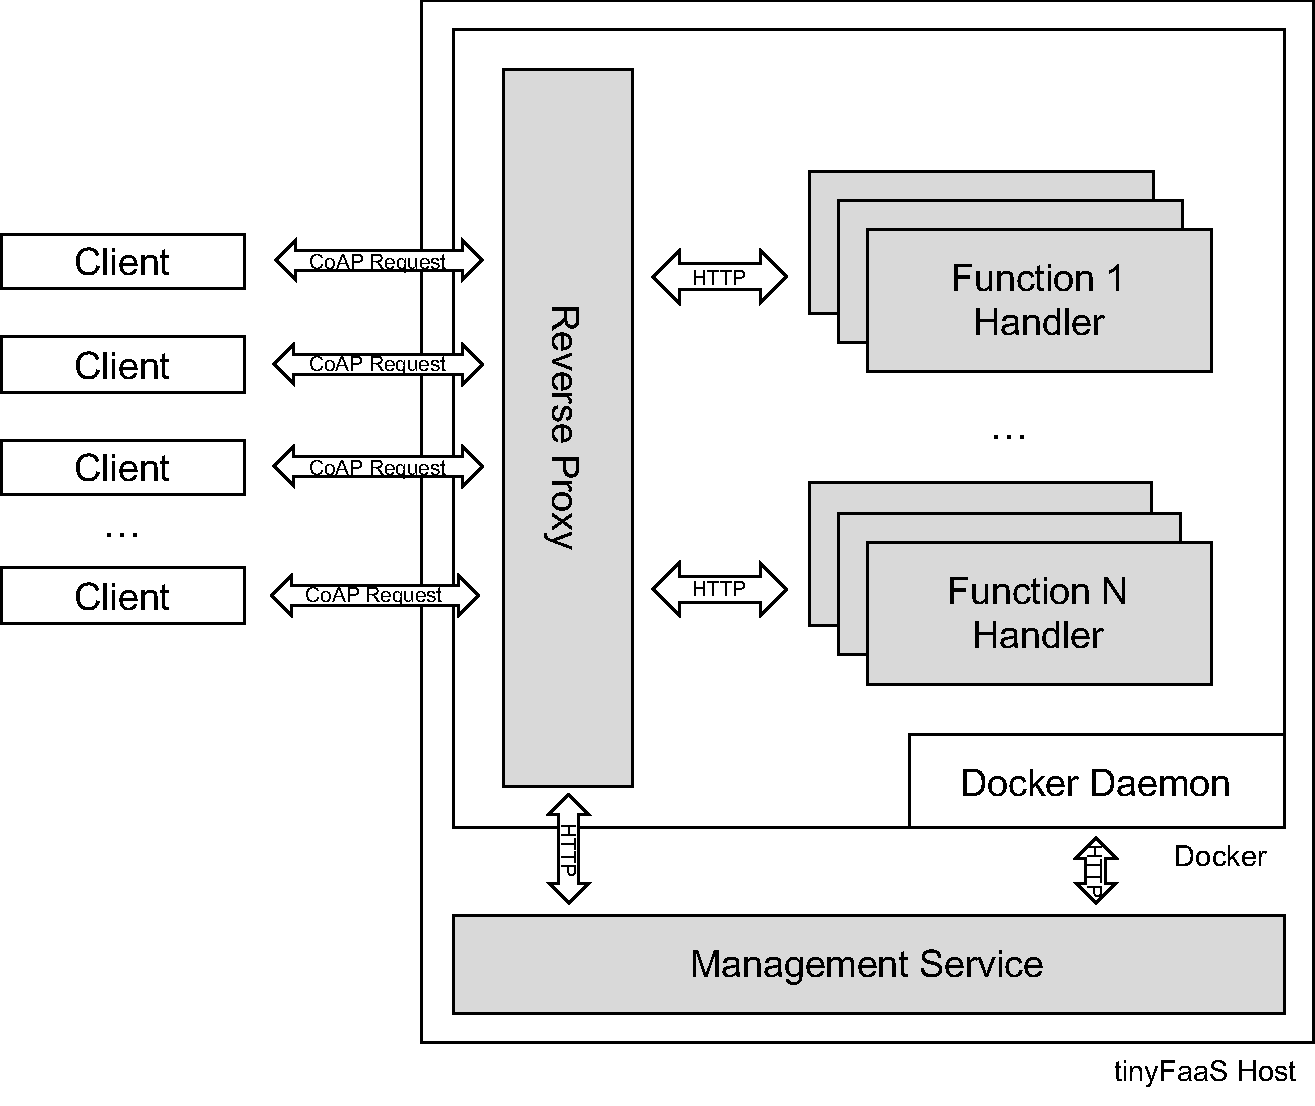
\includegraphics[width=0.66\columnwidth]{fig/architecture.pdf}
  \caption{\textit{tinyFaaS} Architecture}
	\label{fig:systemdesign}
\end{figure}

In this section we will present the architecture of \textit{tinyFaaS}, which is shown in Figure \ref{fig:systemdesign}.
Its main components are a reverse proxy that acts as a CoAP proxy and load balancer, function handlers that execute the application code, and a management service to supervise the other components.

As each of these components communicates using standard web protocols, they are easily interchangeable as well, which further increases extensibility.
For example, the reverse proxy, which accepts incoming CoAP connections, could easily be replaced with an HTTP proxy for less latency-sensitive applications or to integrate it into legacy systems.
While \textit{tinyFaaS} is designed to run on a single node, it is also possible to integrate multiple nodes in a common middleware or through an external load balancer by extending the management service or reverse proxy.

\section{Reverse Proxy}
\label{sec:reverseproxy}

The reverse proxy accepts incoming CoAP connections and proxies them to the function handlers.
For each function, a CoAP resource is registered in the reverse proxy and requests to that resource are treated as a call to the corresponding function.
When a message reaches the CoAP endpoint, the reverse proxy selects one of the function handlers to process this request.
The reverse proxy then sends an HTTP request, possibly with some meta-information or data, to the HTTP proxy in the selected function handler.

As we have discussed in Section~\ref{sec:focus_on_iot}, a FaaS platform for the edge should natively support messaging protocols that are used for machine-to-machine communication and fit the IoT use case as well.
We decided to use CoAP as the messaging protocol for \textit{tinyFaaS} for several reasons.
First, CoAP, which is short for \textit{Constrained Application Protocol} follows the client/server paradigm in the style of HTTP, compared to the publish/subscribe approach that MQTT takes.
This fits our use case as we expect clients such as IoT devices to send requests to the server that hosts \textit{tinyFaaS} without the need for a common message broker.
Second, CoAP is very efficient and lightweight.
All other factors being equal, it introduces much lower latency overheads and can sustain higher throughput levels compared to HTTP and MQTT.
These lower resource needs are mainly due to CoAP using UDP at the transport layer.
As TCP is connection-oriented, it introduces a lot of overhead; UDP, in contrast, does not use a controlled connection between the two communicating parties.
This not only greatly reduces how much processing is needed for each CoAP packet but also reduces network bandwidth usage~\cite{Laaroussi2018-fk,Naik2017-cn}.


\section{Function Handlers}
\label{sec:handlers}

\begin{figure}
	\centering
	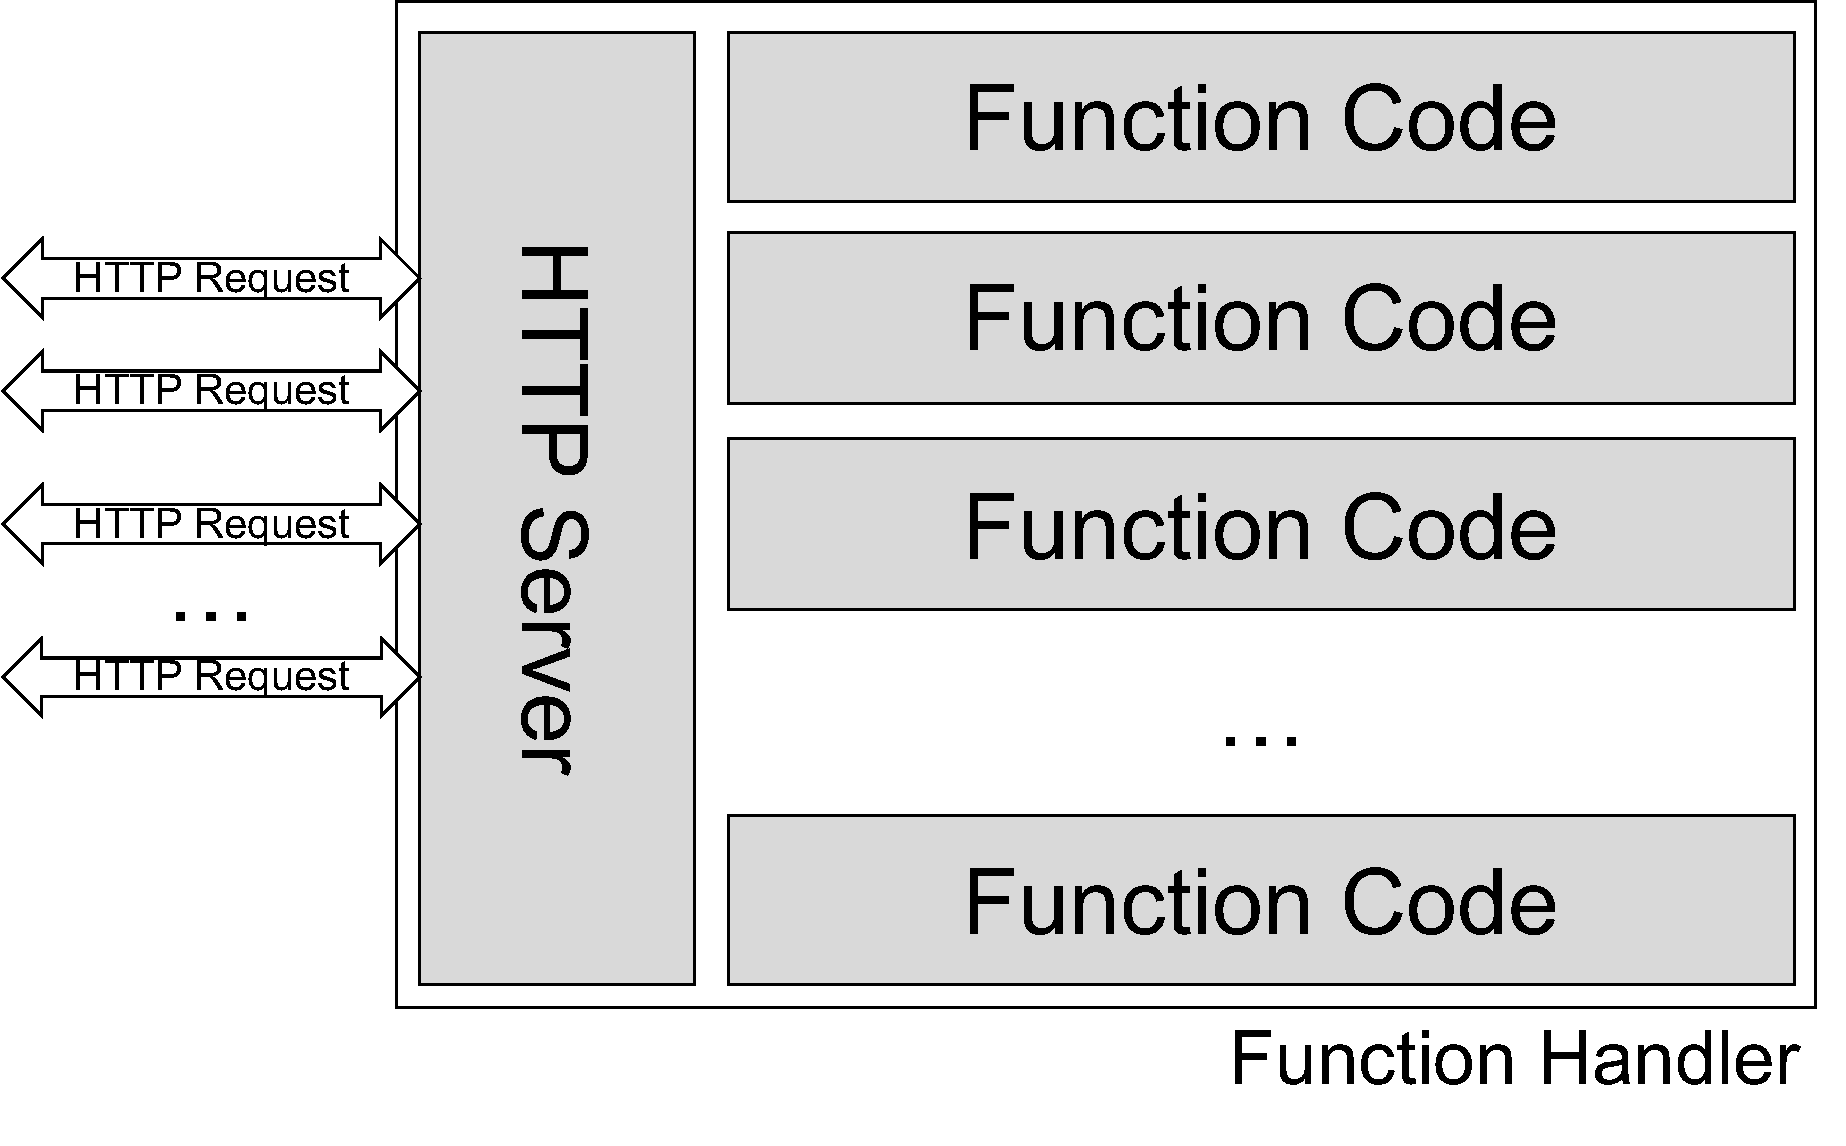
\includegraphics[width=0.66\columnwidth]{fig/functionhandler.pdf}
	\caption{Components of the Function Handler}
	\label{fig:functionhandlers}
\end{figure}

The function handlers are the main part of \textit{tinyFaaS}.
Each function handler is a separate Docker container.
This container contains both a runtime for the programming language that the function is written in and some boilerplate code to facilitate calling it from the reverse proxy.
As shown in Figure \ref{fig:functionhandlers}, the container also includes an HTTP server that accepts incoming requests from the reverse proxy, executes the function with the data provided by the request and returns a result.
While the reverse proxy uses CoAP for external communication, HTTP is used internally within \textit{tinyFaaS}.
Using an HTTP server for communication between the reverse proxy and the function handlers makes it very simple to add new function runtimes, as most modern runtimes support some form of HTTP server out of the box with standard libraries, which is not necessarily the case for CoAP.
Using HTTP here, therefore, improves extensibility.
As the reverse proxy and function handlers run on the same physical host and are connected directly with a virtual network, the communication overhead is negligible.
Furthermore, the connection can be reused for every (internal) request.

Each function handler can accept an arbitrary number of concurrent incoming requests.
Consequently, requests within one container are isolated from each other only on an application level by using threads, yet not on an operating system level.
The trust boundary is set at a function level rather than at request level.
While creating a new Docker container for each request would increase isolation, it results in a considerably higher performance overhead and less efficient resource allocation.
We believe that this is ``good enough'' in terms of a trust model.

Consider the following example: A function developer D develops and deploys a function which is used by users U1 and U2.
In this scenario, neither U1 nor U2 can directly access each other's data without involving D.
D, however, needs to be trusted by both users anyhow as they could leak tenant data in other ways as well.
This only leaves the question of a buggy function that leaks information which, however, cannot be properly exploited by either user as such a bug would go in both directions.
Furthermore, in a stateless programming model, this is also very likely to materialize as a malfunction.

Overall, we believe that this suffices for our purposes; there may, however, be scenarios where more isolation at the cost of performance is needed -- these can simply be addressed by routing requests of the respective user (who is unlikely to attack himself) to a dedicated container.
Nevertheless, this means that applications that run on \textit{tinyFaaS} must be developed for safe memory access so as not to interfere with itself when called concurrently.
Across different functions and, by extension, tenants, \textit{tinyFaaS} asserts isolation using Docker containers.
Through isolated runtimes, different function handlers cannot access other function's memory or files and the virtual networks prevent direct calls between them.
This ensures that no maliciously acting function can interfere with other functions.

While Docker containers only introduce a small performance penalty, they dramatically simplify deployment of functions as the corresponding handlers and dedicated virtual networks can easily be created in an isolated fashion by the management service.

\section{Management Service}
\label{sec:management}

The management service is responsible for creating new functions within the platform.
Developers who want to deploy a new function can send it the management service' HTTP endpoint.
The service then creates the containers for the function handlers, registers a CoAP resource in the reverse proxy, and connects all handlers with the reverse proxy on a Docker virtual network so that they can communicate.
In a similar manner, functions may also be updated or deleted.
This allows functions on \textit{tinyFaaS} to be reconfigured at runtime, which is a key feature of FaaS platforms.

Furthermore, having a single point of entry also enables multi-tenancy as the management service can take care of user authentication when creating or modifying functions.
While it would be possible to integrate this into the reverse proxy, as we tried in an earlier prototype, having the management service as a separate component has two advantages.
First, it keeps the reverse proxy as slim as possible, making it more resource efficient.
Second, having separate components allows us to replace individual components.
For instance, it is possible to configure \textit{tinyFaaS} by sending HTTP requests to the host's Docker daemon and the existing \textit{tinyFaaS} reverse proxy.
This allows us to easily replace the management service, e.g., with an external or distributed service which would add remote management capabilities to our system.

\chapter{Evaluation}
\label{cha:evaluation}

We evaluate our approach through (i)~a proof-of-concept implementation and (ii)~a number of experiments in which we assess performance overheads of \textit{tinyFaaS} and compare it to two alternative approaches from related work.

\section{Proof-of-Concept Implementation}
\label{sec:implementation}

As described, \textit{tinyFaaS} comprises three main components: the reverse proxy, the function handlers, and the management service.
For simplicity, in our proof-of-concept, only a Node.js v8 runtime is supported.
The function handlers are Docker containers running a Node.js script with an HTTP endpoint that accepts any incoming requests using the \texttt{http} module.
The actual function code is loaded as a module to that script and its exposed function is executed for each incoming request.

The management service is a Python3 application that uses \texttt{docker-py} to manage the Docker containers, images, and networks needed for \textit{tinyFaaS}.
It exposes an HTTP endpoint for us to add new functions to \textit{tinyFaaS}.
When a new function is created, the management service creates a configurable number of Docker containers that each contains a function handler for the function.
For each function, it also creates a dedicated Docker network to which it attaches all function handlers and the reverse proxy.

We implemented the reverse proxy in Go, using the \texttt{go-coap} library.
The reverse proxy accepts incoming HTTP requests from the management service to create a new CoAP resource with a given identifier and given IP addresses of existing Docker containers on the \textit{tinyFaaS} host that incoming CoAP requests should be forwarded to.
The small binary that the reverse proxy compiles to is then also run in a Docker container.
Our implementation is available as open-source software\footnote{https://github.com/OpenFogStack/tinyFaaS}.

\section{Experiment Setup}
\label{sec:experiment}

In our experiments, we compared \textit{tinyFaaS} to both an existing edge FaaS platform and a high-performance cloud FaaS platform.
We also assessed the \textit{tinyFaaS} overhead by comparing its performance to the performance of a native, non-dockerized Node.js deployment on the same machines.
This native implementation also uses a CoAP endpoint, which should help us understand how the internal design of \textit{tinyFaaS} affects performance rather than the use of a more efficient communication protocol.
For this, we attached a \texttt{node-coap} server.
As an edge FaaS platform, we use Lean OpenWhisk which is a deployment option of the OpenWhisk platform that targets resource constrained systems\footnote{https://www.github.com/kpavel/incubator-openwhisk/tree/lean}.
For the cloud FaaS platform, we use Kubeless which is based on Kubernetes\footnote{https://kubeless.io/} and has recently been shown to be one of the most efficient open-source FaaS platforms.
As such it is a good candidate for edge deployment.
Furthermore, as it has been shown to be more efficient than OpenFaaS or Knative, we refrain from benchmarking these platforms as results are fairly predictable based on the experiments of~\cite{Palade2019-mo}.
For the Kubeless experiments, we used a minikube\footnote{https://minikube.sigs.k8s.io/} installation.
For the workload, we implemented a custom JavaScript function that computes the prime numbers between 1 and 1,000 using the \textit{Sieve of Eratosthenes}~\cite{sieve} algorithm and deployed it on \textit{tinyFaaS}, Kubeless, Lean OpenWhisk, and natively.

As we target edge environments, we use single node deployments.
We select a Raspberry Pi 3 B+ and an AWS EC2 m5a.large virtual machine as our hardware to test the performance both on a very constrained single-board computer and a more powerful server, in this case the moderately powerful general-purpose cloud server available on AWS EC2 that is comparable to a single-node edge server.
The Raspberry Pi 3 B+ has a quad-core 1.4GHz processor, 1GB of memory, and a 300 Mbps Ethernet connection running the recommended Raspbian Buster distribution\footnote{https://www.adafruit.com/product/3775}.
The AWS EC2 m5a.large instance provides two vCPUs of the AMD EPYC 7000 series, 8GB of memory, and up to 10Gbps of bandwidth\footnote{https://aws.amazon.com/ec2/instance-types/m5/}.

For the workload generation, we implemented a custom benchmarking tool on Node.js that supports both CoAP and HTTPS, which is necessary when comparing \textit{tinyFaaS} to Lean OpenWhisk and Kubeless, which both only support HTTPS triggers.
While comparing latency measurements may be inaccurate based on the different implementations of the native Node.js \textit{https} and the third-party \textit{node-coap} libraries, we expect the differences to be in favor of \textit{https}, i.e., in favor of Lean OpenWhisk and Kubeless.
The benchmarking tool itself follows a closed workload model~\cite{paper_schroeder_open_closed_workloads,book_bermbach_cloud_service_benchmarking} and issues a sequence of calls to a target endpoint using a configurable number of client threads as in YCSB~\cite{paper_cooper_ycsb}.
For the Raspberry Pi experiments, we run the benchmarking client on a MacBook Air and connect both machines with an Ethernet uplink.
For the cloud server benchmark, we use an AWS EC2 m5a.xlarge server that is more powerful than the system under test.
Both cloud servers are located in the same availability zone in the EU Central AWS region.
For all experiments, we asserted that the machine running the benchmark client did not become a bottleneck~\cite{book_bermbach_cloud_service_benchmarking}.

To measure the performance of the target platforms under different load levels, we varied the number of client threads.
We used 1, 4, 16, 64, 256, and 1024 client threads for all experiments.
Each client thread issues a total of 500 operations which each trigger one execution of our example function.
We repeat all experiments three times to assert reproducibility of results, but only report the run with the median average latency.
All repetitions yielded comparable results.


\section{Experiment Results}
\label{sec:discussion}

\begin{figure*}[ht]
  \centering
  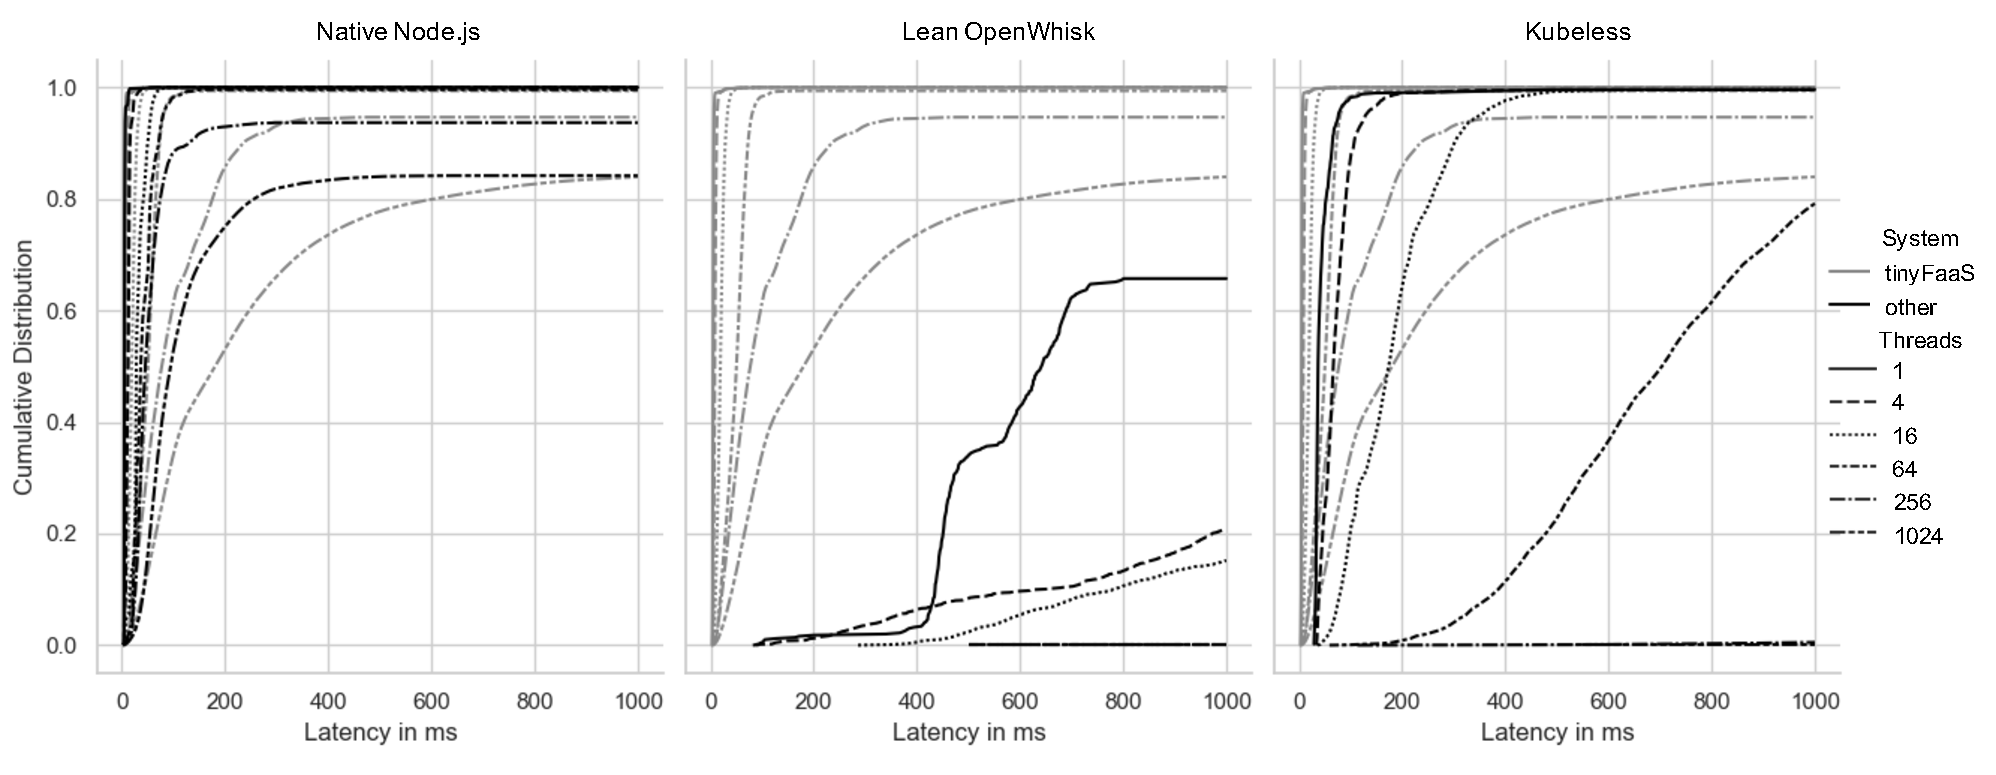
\includegraphics[width=1\columnwidth]{fig/pigraph.pdf}
  \caption{Latency Measurements on Single-Board Computer}
  \label{fig:pigraph}
\end{figure*}

\begin{figure*}[ht]
  \centering
  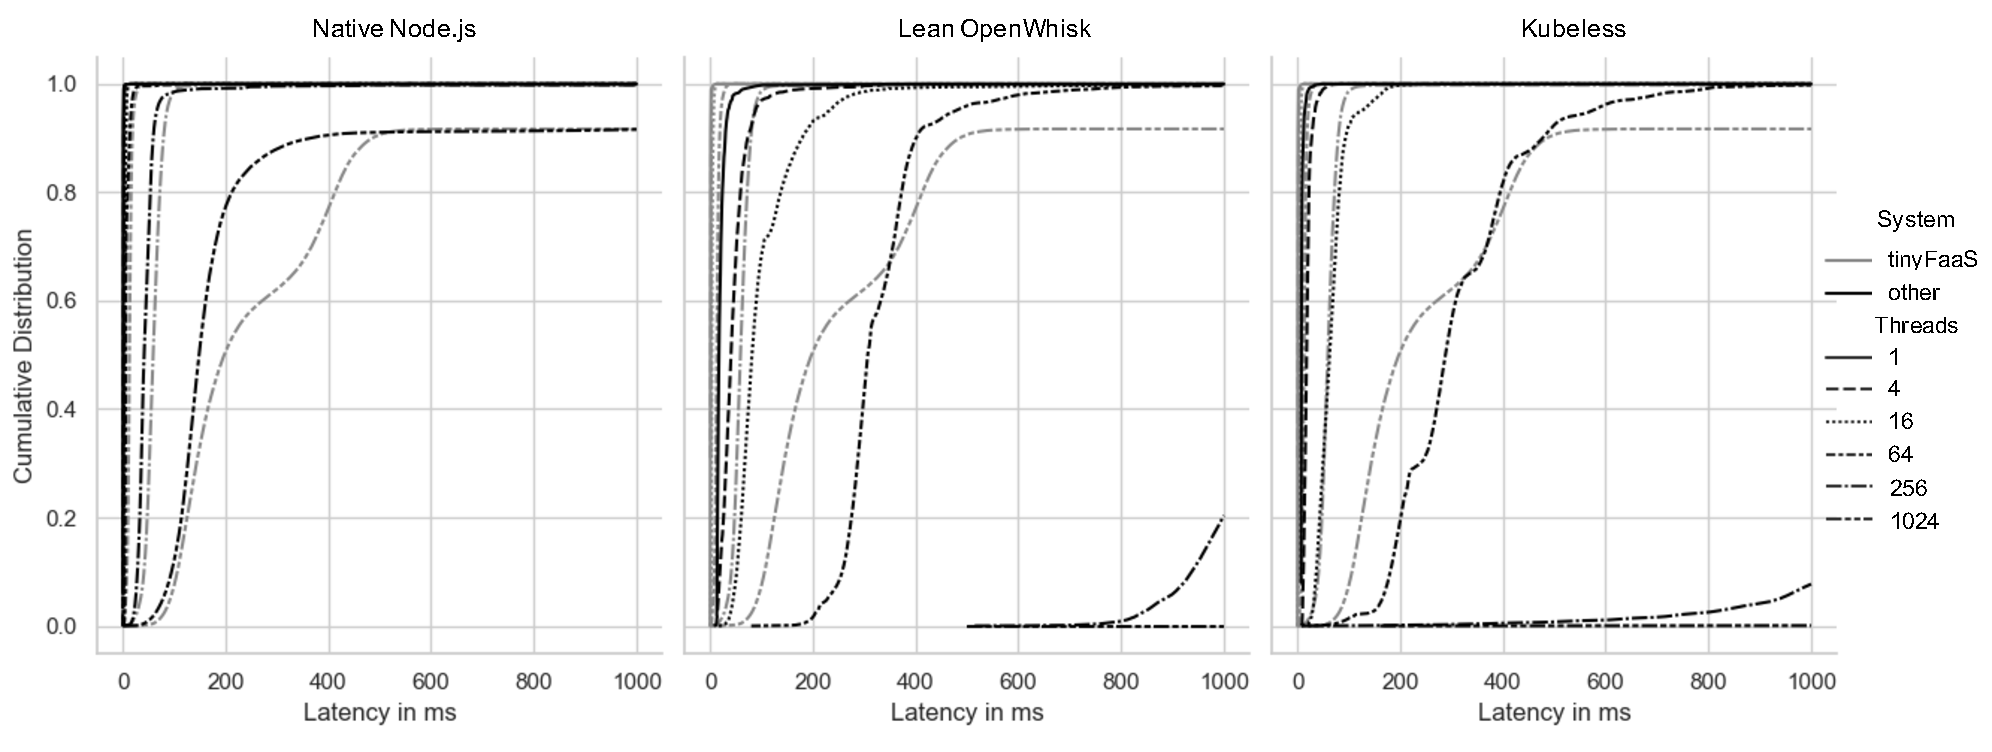
\includegraphics[width=1\columnwidth]{fig/awsgraph.pdf}
  \caption{Latency Measurements on Cloud Server}
  \label{fig:awsgraph}
\end{figure*}

In our experiments, we find that the best case average execution time for our exemplary function is 6ms on the single-board computer and 1ms on the cloud server.
These values are taken from the test against the native Node.js implementation using a low load of one parallel request.
For our results, we consider all operations that do not return any response and those with a response time of more than one second as failed.

\textbf{Overhead of tinyFaaS:} Figure \ref{fig:pigraph} and Figure \ref{fig:awsgraph} show the cumulative distribution of the respective latency measurements.
Please, note that this also shows the success rate for each experiment.
We show the measurements for \textit{tinyFaaS} along with each of the systems we compare it to, namely the native Node.js implementation, Lean OpenWhisk, and Kubeless.
As each client thread in our benchmarking tool only sends a new request when it receives a response or the previous request times out, throughput varies across all experiments.
We achieve the highest throughput of 9,800 operations per second with the native Node.js implementation on the Raspberry Pi with 1024 simultaneous connections.
On average, the benchmarking client issues a load of 38 operations per second per client thread on the Raspberry Pi and 172 operations per second per client thread on the cloud server.

Figure \ref{fig:pigraph} shows that performance of \textit{tinyFaaS} is comparable to the native deployment on the Raspberry Pi.
Especially the success rates being equal shows that both scale equally well and that \textit{tinyFaaS} introduces a low to acceptable overhead.
At small scale both perform equally well in terms of response latency.
In fact, in our tests with 16 simultaneous client connections, \textit{tinyFaaS} outperforms by 59\%.
We expect this to be caused by the implementation of CoAP in Node.js compared to our use of HTTP within our Node.js function handlers.
Furthermore, using multiple function handlers could help distribute load more evenly across CPU cores which Node.js by default does not do without explicitly designing for multithreading.
Nevertheless, for high loads the native implementation is about 40\% faster than \textit{tinyFaaS}.
As shown in Figure \ref{fig:awsgraph}, results look similar in our cloud server experiments.
Unlike the single-board computer experiments, these do not show \textit{tinyFaaS} outperforming the native implementation at low load.
The reason for this might be that the cloud server has only two available CPU cores, albeit much more powerful ones, which could limit the impact of the multithreading advantage.
On average, the native implementation is 8\% faster than \textit{tinyFaaS} for small loads and 33\% faster with a medium to high load.

\textbf{tinyFaaS vs. Lean OpenWhisk:} Lean OpenWhisk on a constrained system as our Raspberry Pi is much slower than \textit{tinyFaaS} and scales considerably worse.
Even with just a single concurrent connection Lean OpenWhisk is unable to successfully respond to about two thirds of all requests.
In addition, the average latency for successful requests is almost 100 times as high as for \textit{tinyFaaS}.
With 256 and 1024 client threads, Lean OpenWhisk on our single-board computer fails completely with no successful response to any request.
In fact, we observed that the Raspberry Pi would not accept any more input at all and needed to be reset after each test.
We presume that the high memory usage of Lean OpenWhisk led to swapping which in turn put a high demand on the processor.
On the cloud server, results look slightly better for small to medium loads.
Lean OpenWhisk is able to successfully respond to all requests, albeit with a latency that is 20 times higher than that of \textit{tinyFaaS}.
Despite that, unlike \textit{tinyFaaS}, Lean OpenWhisk is not able to scale beyond 256 client threads.

\textbf{tinyFaaS vs. Kubeless:} Kubeless scales better than Lean OpenWhisk on the constrained Raspberry Pi but still has about 20\% error rate even under medium load.
At higher load levels, it also fails completely, i.e., does not return any results.
Response latency for Kubeless is better than Lean OpenWhisk, yet on average still more than eight times as high as the latency of \textit{tinyFaaS}.
We did expect Kubeless to be more powerful than Lean OpenWhisk based on~\cite{Palade2019-mo}, nonetheless Kubeless and Minikube do seem to introduce considerable overhead.
Furthermore, some part of that overhead can likely be attributed to the use of HTTP instead of the more efficient CoAP.
Results for the cloud server experiments appear comparable, with the exception of Kubeless scaling up a bit further, which is expected given the more powerful hardware.
On average, Kubeless is 13 times slower than \textit{tinyFaaS} in these measurements.

These benchmark results reveal some important insights about the performance of \textit{tinyFaaS}.
Even though our proof-of-concept lacks more advanced features such as a more intelligent scheduling and container management, it was able to beat Lean OpenWhisk and Kubeless in throughput and scalability.
The performance difference is especially apparent when running these platforms on resource constrained hardware such as our Raspberry Pi.
As in an edge computing environment performance on constrained, single node devices is crucial, this shows that \textit{tinyFaaS} is the better fit for such environments.

\chapter{Related Work}
\label{cha:relatedwork}

While Function-as-a-Service is still a relatively new paradigm, it has found widespread interest, in particular as a cloud service.
Next to the popular AWS Lambda and Azure Functions, a number of open-source approaches have been developed for the cloud, e.g., the already mentioned OpenWhisk and Kubeless.

There are also some attempts at FaaS platforms for the edge.
OpenWhisk for example has Lean OpenWhisk as a deployment option that removes a lot of resource-intensive components such as a Kafka queue, that are needed to scale across multiple nodes~\cite{Breitgand2018-fs}.
Amazon and Microsoft have also already started bringing their FaaS platforms closer to the edge of the network with AWS Greengrass\footnote{https://aws.amazon.com/greengrass} and Azure Functions on IoT Edge\footnote{https://docs.microsoft.com/azure/iot-edge}, which promise seamless integration into the respective cloud ecosystems.
To use these services, however, developers need to render control of the edge device to the cloud service provider.

Palade et al.~\cite{Palade2019-mo} have published a comparison of open-source FaaS platforms for the edge using qualitative as well as quantitative measures.
The authors also compare OpenWhisk, yet not Lean OpenWhisk, OpenFaaS\footnote{https://www.openfaas.com/}, Kubeless, and Knative\footnote{https://knative.dev/}.
They find that OpenWhisk has by far the worst performance of the four, especially with an increased load, while Kubeless provides the highest throughput and lowest latency across all quantitative tests.

Recently, Akkus et al.~\cite{Akkus2018-gj} have published an approach for high-performance serverless computing that is similar to \textit{tinyFaaS} conceptually.
To allow for quicker communication between functions and limit the overhead of Docker, their system allows for concurrent execution of functions within a single container and grouping applications that consist of several functions.
With their approach, they were able to achieve a 43\% speedup compared to OpenWhisk whereas our results showed improvements of at least 2,000\%.

Beyond these related research efforts, Hussain et al.~\cite{Hussain2019-mj}, Cicconetti et al.~\cite{Cicconetti2018-hw}, Baresi et al.~\cite{Baresi2017-jg}, Nastic et al.~\cite{Nastic2018-ec}, and more have all described more general serverless frameworks for the edge but they do not directly address lightweight FaaS platform for edge computing environments.
These approaches, hence, seem incompatible with installation on low power edge devices.

Rausch et al.~\cite{Rausch2019-eo} propose and implement a serverless platform for AI applications at the edge that combines placing execution on edge nodes and handling data in a locality-aware manner.
Data such as AI models can be pulled from the cloud or another edge node, while the serverless platform abstracts from any data management by providing data proxies.
Furthermore, they also propose a centralized scheduler that is able to extend to the edge if needed.
This scheduler could schedule function calls across many different edge node clusters while taking hardware capabilities of different nodes into consideration.

In~\cite{Shillaker2018-di}, Shillaker lays out their plans to develop an edge serverless framework for low-latency applications.
They find that OpenWhisk is not sufficient in its performance, especially when scaled, and recommends improving the runtime, scheduling, and state sharing.
Instead of using Docker containers, Shillaker's approach is to use language runtimes to provide isolation while also introducing as little performance overhead as possible.
Building on top of that function runtime, they also propose improving on the relatively simple existing FaaS platform schedulers with a custom one that considers resource sharing within the runtime.
And, finally, the author aims to introduce state management into their serverless platform, which they suggest can broaden its application areas as also hinted at by Hellerstein et al.~\cite{paper_hellerstein_serverless}.

Similarly, Hall et al.~\cite{Hall2019-im} argue that containers are not fit for serverless at the edge, as they introduce unnecessary delays during container startup, and their nonmalleable resource assignments hinder efficient resource usage.
Their solution is to use a WebAssembly runtime instead, which can also provide both sandboxing, memory safety, and interoperability.
Currently the WebAssembly approach can remedy cold-start overheads but performance is worse than in OpenWhisk.

Karhula et al.~\cite{Karhula2019-en} describe an edge FaaS platform based on Docker that allows for checkpointing of functions, pausing the execution of a function, and taking a snapshot of the container at a particular instance in time.
This enables pausing long-running or blocking functions when resources are needed, backing up functions in case of failures, and even for container state migration across different platform nodes.
While their experiments do show that checkpointing containers introduces a latency overhead compared to paused containers, their memory footprint is much smaller.

\chapter{Conclusion}
\label{cha:conclusion}
Serverless is a very promising paradigm for the edge as resources can be allocated in time slices (functions) instead of long-running containers or virtual machines.
As edge nodes, however, are often resource constrained, a serverless edge platform needs to be rather lightweight which is not the case in current (cloud-focused) open-source FaaS systems.

To address this gap, we have presented \textit{tinyFaaS}, a lightweight, single-node FaaS platform for edge environments.
Using CoAP as application protocol and intelligent sharing of function containers, \textit{tinyFaaS} is able to achieve the desired properties.
For our evaluation, we implemented a proof-of-concept prototype and ran a number of experiments in which we compared the performance of our prototype to Lean OpenWhisk (the only edge-focused open-source FaaS platform that we are aware of) and Kubeless (the most resource efficient open-source FaaS platform~\cite{Palade2019-mo}).
While our experiments show that a native implementation can still be 40\% faster than our \textit{tinyFaaS} prototype, we also show that \textit{tinyFaaS} is 20 to 100 times faster than Lean OpenWhisk and 10 times faster than Kubeless.
Our experiments also show that \textit{tinyFaaS} scales just as well as a native deployment and significantly better than both Lean OpenWhisk and Kubeless.


% Include more chapters as required.

%%=========================================
%Backmatter

\appendix
%!TEX root = ../thesis.tex

\cleardoublepage
\chapter{Technologies and Concepts of a Larger Context}

This appendix chapter contains definitions for technologies and concepts that are mentioned in the thesis, but are not of higher importance for it. Section \ref{sec:paxos} introduces a consensus algorithm for distributed systems.

\section{Finding Consensus in a Distributed System}
\label{sec:paxos}

The Paxos algorithm has first been described by Leslie Lamport in his work about the parliament on the island of Paxos \cite{paxos1998}. The parliament's part-time legislators had been able to maintain consistent copies of their records by following the algorithm protocol.  While the original work's main focus has not been the application in computer science, the author simplified his explanations later in \cite{paxos2001} and described how Paxos can be used to find consensus in fault-tolerant distributed systems.

Even though the Paxos algorithm cannot mitigate Byzantine failures (see appendix \ref{app:dic}), it can mitigate the effects of different processing speeds of participants and reordered, delayed, or lost messages. The only requirement is that at least half of the participants can somehow communicate.

In Paxos, four different roles exist. The \textbf{client} issues requests and waits for responses. Based on the client's request, multiple \textbf{proposer} propose a value. All these proposals are processed by the \textbf{acceptors} which will agree upon one at the end. Finally, there are the \textbf{learners} which guarantee persistence of agreed decisions and respond to client reads. The usual setup used in practice, in which every machine participating fulfills each of the roles besides the client role, is shown in figure \ref{fig:paxosSetup}.

\begin{figure}[ht]
    \centering
	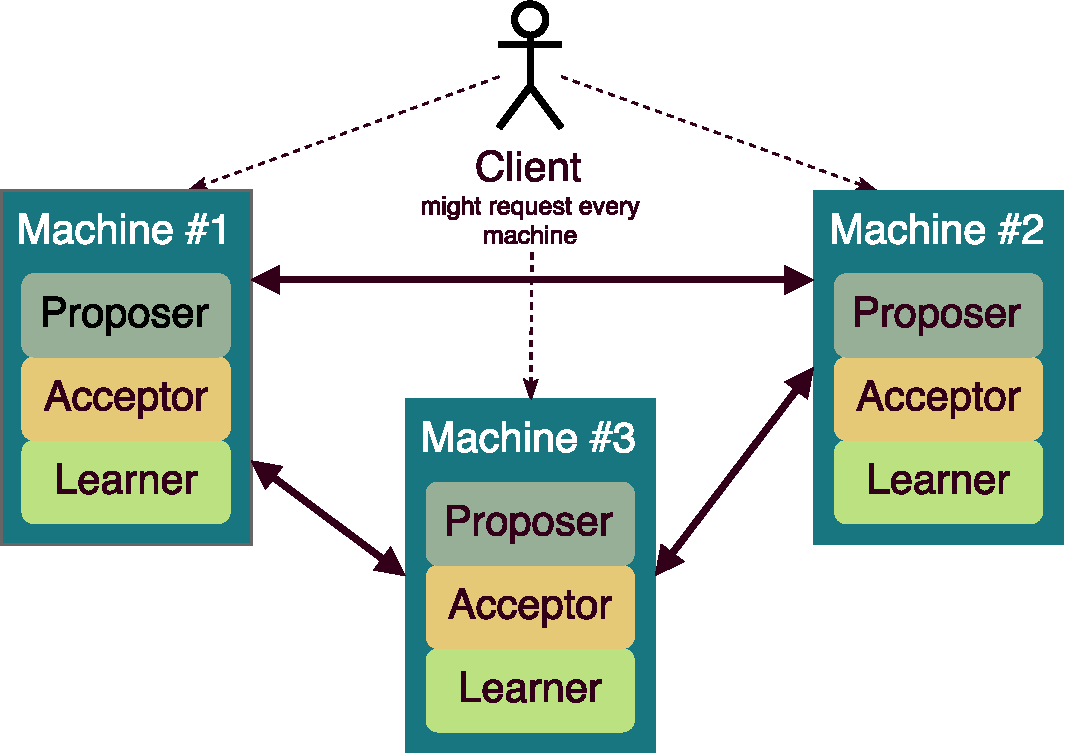
\includegraphics[width=0.8\textwidth]{fig/PaxosSetup.pdf}
	\caption{Example Setup of Three Machines Agreeing on Values Based on the Paxos Algorithm}
	\label{fig:paxosSetup}
\end{figure}

\section{Detecting Mutual Inconsistency}
\label{sec:versionVector}

Parker et al. claim that a system must ensure the mutual consistency of data copies by applying all changes made to one copy to all others correspondingly \cite{versionVektor}. Each time two copies of the same original data item have a different set of modification applied to them, they become incompatible and this conflict must be detected. However, this is not trivial, because \enquote{network partitioning can completely destroy mutual consistency in the worst case}. Nevertheless, Parker et al. state that the efficient detection of conflicts that lead to mutual inconsistency can be done by a concept they call \textit{version vectors}. They define a version vector for an item f as \enquote{a sequence of n pairs, where \textit{n} is the number of sites at which f is stored. The \textit{i}th pair ($S_i$: $v_i$) gives the index of the latest version of \textit{f} made at site $S_i$}. An example vector for an item stored at the sites A, B and D is $<$A:2, B:4, D:3$>$, which translates in a file that has been modified twice on site A, four times on site B, and thrice on site D.

A set of vectors is \enquote{compatible when one vector is at least as large as any other vector in every site component for which they have entries}. Otherwise the vectors conflict and are incompatible. E.g., the two vectors $<$A:2, B:4, D:3$>$ and $<$A:4, B:5, D:3$>$ are compatible because the second one dominates the other one. $<$A:3, B:4, D:3$>$ and $<$A:2, B:5, D:3$>$ conflict, because the first one indicates that the data item was modified one more time on node A, while the second one indicates one more modification occurred on node B. However, if we add a third vector $<$A:3, B:5, D:4$>$, no conflict exists anymore, because it dominates the two others. The consequences of an operation performed on a data item for a data item's vector is depicted in table \ref{tab:vectorOperations}.

\begin{table}[ht]
    \centering
    \begin{tabularx}{\linewidth}{@{}>{\bfseries}l@{\hspace{.5em}}X@{}}
        \toprule
        \textbf{Operation related to data item} & \textbf{Consequence for vector of data item}\\ \midrule
        Update on site $S_i$ & Increment $v_i$ by one\\
        Delete or rename on site $S_i$ & Keep vector and increment $v_i$ by one, remove data item value\\
        Reconcile version conflict & Set each $v_i$ to maximum $v_i$ from all vectors used for reconciliation. In addition, increment $v_i$ of site that initiated reconciliation by one\\
        Copy to new site & Augment vector to include new site\\
        \bottomrule
    \end{tabularx}
    \caption{Influence of Operations on a Data Item's Version Vector}
    \label{tab:vectorOperations}
\end{table}

By using version vectors, one can detect version conflicts and initiate (automatic) reconciliation. However, Parker et al. warn that two identical updates made on separate partitions will result in a conflict, even though none is present. Thus, they recommend to additionally check two data items on differences before a conflict is raised in certain applications. Furthermore, the reconciliation is most times not trivial, that's why tools such as Cassandra delegate this task to the application layer \cite{cassandra2010}.

%!TEX root = ../thesis.tex

\cleardoublepage
\chapter{Acronyms}
\begin{description}
\item[AWS] Amazon Web Services
\item[IoT] Internet of Things
\end{description}

%!TEX root = ../thesis.tex

\cleardoublepage
\chapter{Lexicon}
\label{app:dic}

\paragraph*{Byzantine failure} A malfunction of a component that leads to the distribution of wrong/conflicting information to other parts of the system is called Byzantine failure \cite{lamport1982byzantine}. The name is based on the Byzantines Generals Problem, in which three Byzantine generals need to agree on a battle plan while one or more of them might be a traitor trying to confuse the others.

%!TEX root = ../thesis.tex

\cleardoublepage
\chapter{Listings}
\label{app:listings}

This is the appendix for code, that does not need to be provided directly inside the thesis.

\section{Configuration for Node A}

\lstinputlisting[style=json, caption={Configuration for Node A}, label={lst:nodeAConfig}]{listings/nodeAConfig.js}

% Include more appendices as required.

\cleardoublepage
\addcontentsline{toc}{chapter}{Bibliography}
\defbibheading{notonline}{\chapter*{Bibliography}}
\printbibliography[heading=notonline]

%%=============================================

\end{document}
